%\documentclass[smalldemyvopaper,11pt,twoside,onecolumn,openright,extrafontsizes]{memoir}
\documentclass[20pt,twoside,openright,extrafontsizes,landscape]{memoir}
\usepackage{yfonts,color,hyperref}
\def\initdefault{yinit}
\usepackage[utf8x]{inputenc}
\usepackage{fontspec}
\usepackage[spanish]{babel}
\usepackage{xsavebox} %save content for repeated use
\usepackage{atbegshi} %insert material on every page
\usepackage[x11names,dvipsnames]{xcolor} 
\usepackage{wrapfig}  
\usepackage{tikz}
\usepackage[tmargin=3cm,bmargin=3cm,lmargin=2cm,rmargin=2cm]{geometry}
%\usepackage[margin=1cm]{geometry}% for screen preview
\usepackage{graphicx}
\setmainfont{juan_letra_reg}
%\DeclareFontFamily{LYG}{OldNewspaperTypes}{}
	
\AtBeginShipout{
	\AtBeginShipoutUpperLeft{\raisebox{-\height}{\xusebox{PageBGPicture}}}
}
\tolerance=1
\emergencystretch=\maxdimen
\hyphenpenalty=10000
\hbadness=10000
\begin{document}

%		\begin{tikzpicture}
%			\node [ minimum width=.\paperwidth, minimum height=\paperheight] () {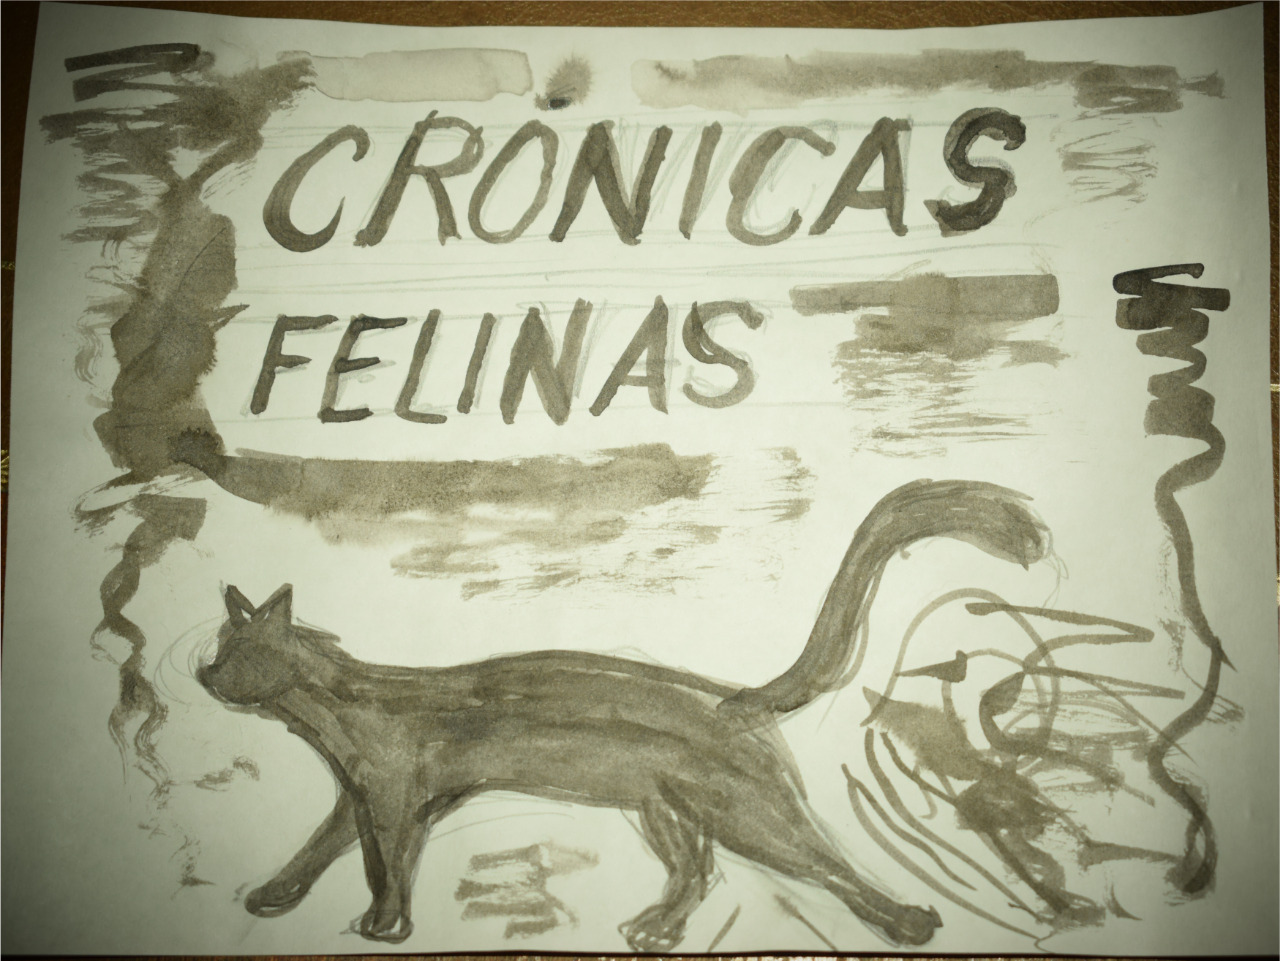
\includegraphics[width=\paperwidth,height=\paperheight,angle=180]{portada}};
%		\end{tikzpicture}
	
%		\begin{tikzpicture}
%	\node [ minimum width=.\paperwidth, minimum height=\paperheight] () {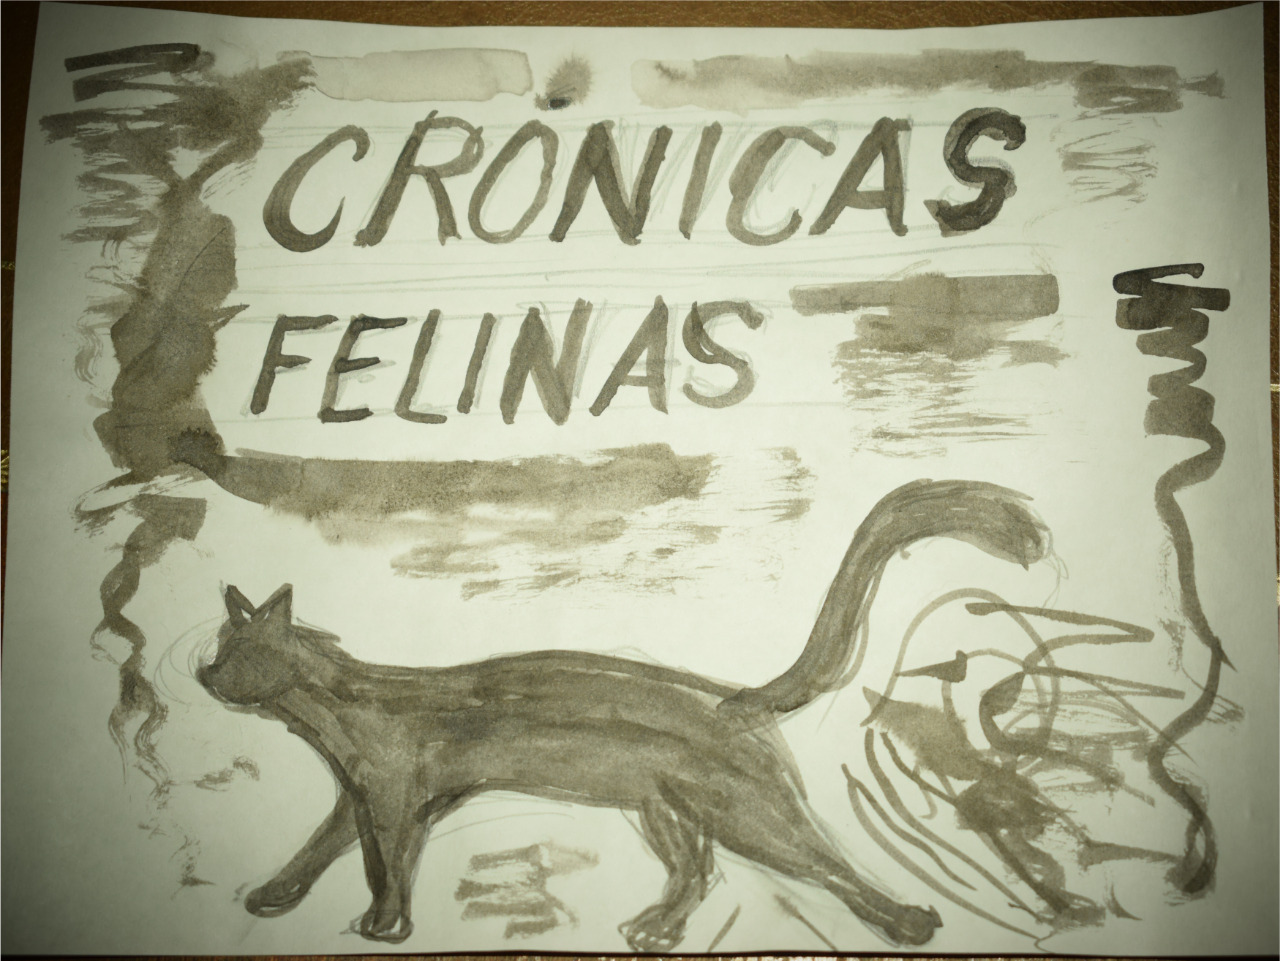
\includegraphics[width=\paperwidth,height=\paperheight,angle=0]{portada}};
%\end{tikzpicture}	

		\xsavebox{PageBGPicture}{%
		\begin{tikzpicture}
		\node [ minimum width=.\paperwidth, minimum height=\paperheight] () {
\includegraphics[width=\paperwidth,height=\paperheight,angle=180]{paper0}};
		\end{tikzpicture}
	}
	\AtBeginShipout{
	\AtBeginShipoutUpperLeft{\raisebox{-\height}{\xusebox{PageBGPicture}}}
}	
\pagenumbering{gobble}
\tikz[remember picture,overlay] \node[opacity=0.8,inner sep=0pt] at (current page.center){
\includegraphics[width=\paperwidth,height=\paperheight,angle=180]{paper0}};	
%\begin{Large}
 \begin{wrapfigure}{r}{5.5cm}
 	
\includegraphics{paper}
 \end{wrapfigure}
\begin{flushleft}
HOLA, MI NOMBRE ES OTTOKO, VIVO EN VILLA DEVOTO. 

SI BIEN PUEDE PARECERLES QUE LLEVO UNA VIDA APACIBLE Y HASTA UN TANTO PEREZOSA, VOY A CONTARLES LA ÚLTIMA DE MIS INTRÉPIDAS AVENTURAS.	
\end{flushleft}
\newpage

\xsavebox{PageBGPicture}{%
	\begin{tikzpicture}
	\node [ minimum width=.\paperwidth, minimum height=\paperheight] () {
\includegraphics[width=\paperwidth,height=\paperheight,angle=180]{paper1}};
	\end{tikzpicture}
}
%	\AtBeginShipout{
%	\AtBeginShipoutUpperLeft{\raisebox{-\height}{\xusebox{PageBGPicture2}}}
%}	
\pagenumbering{gobble}
\tikz[remember picture,overlay] \node[opacity=1,inner sep=0pt] at (current page.center){
\includegraphics[width=\paperwidth,height=\paperheight,angle=180]{paper1}};
\begin{tikzpicture}
\node[] (hoja_2) {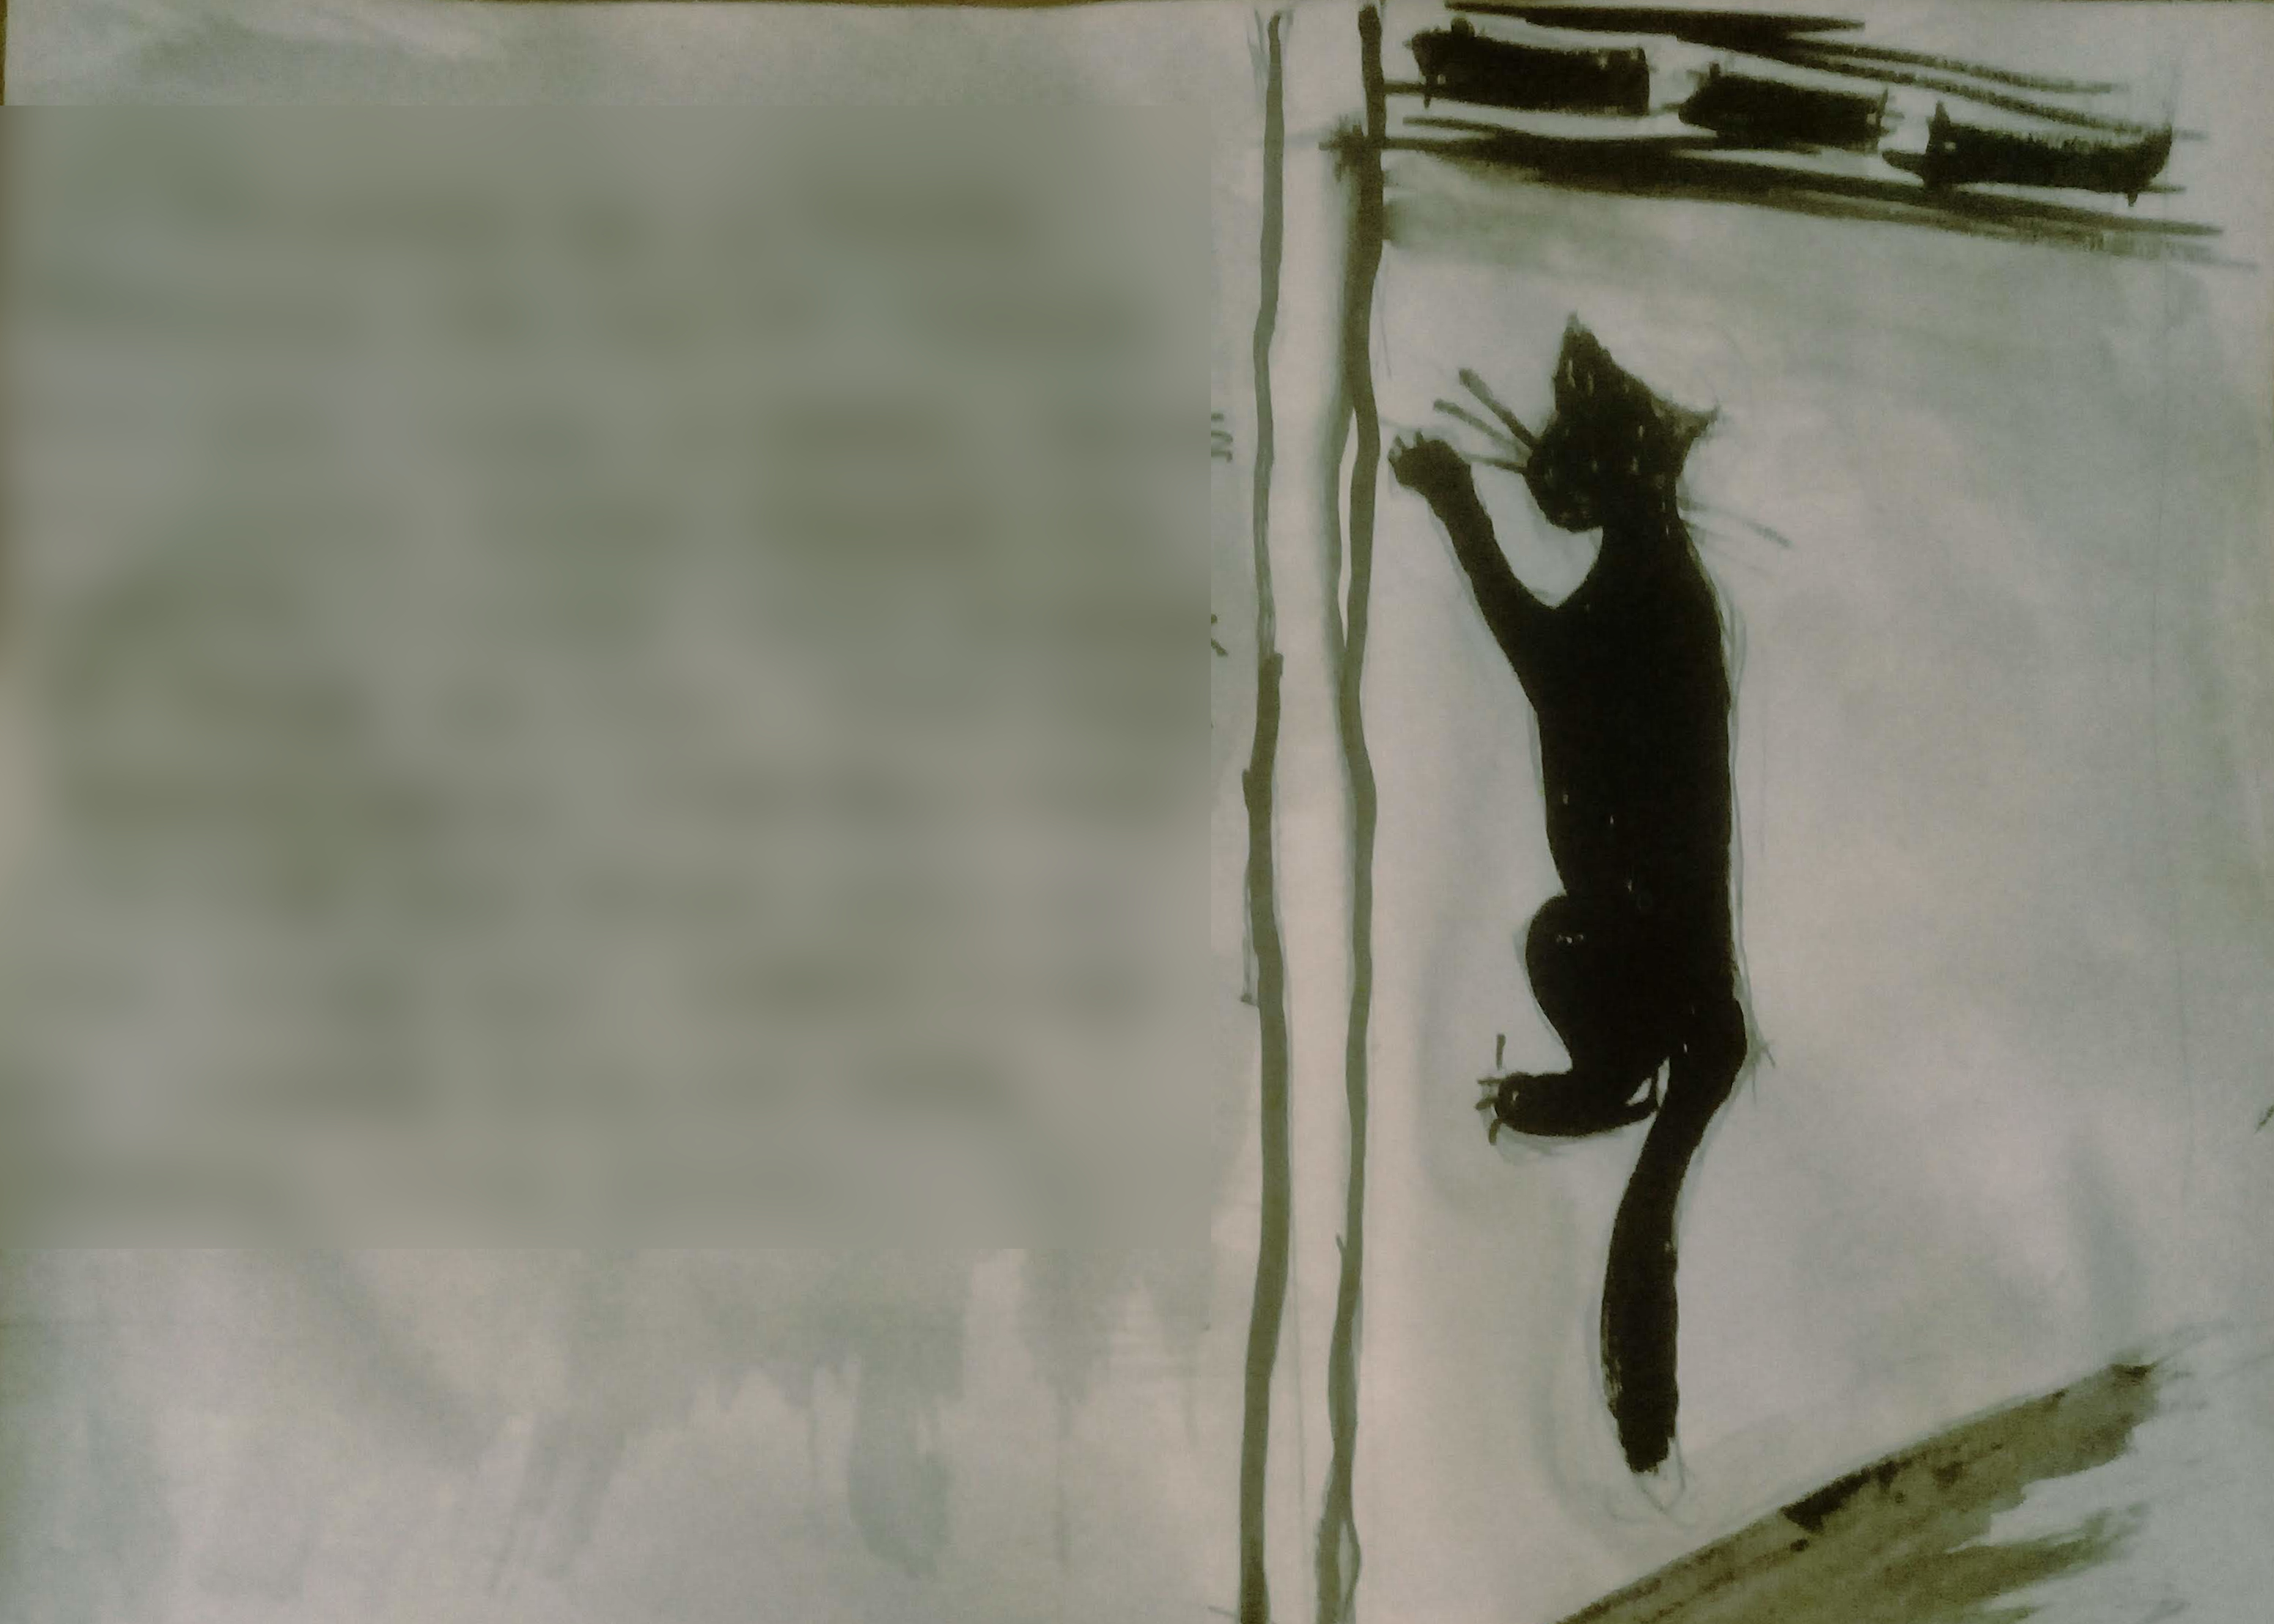
\includegraphics[width=.91\textwidth]{trepando_pared}};
\node[text width=11cm,xshift=-4cm] at (hoja_2){EL RECUERDO DE LA PALOMA BURLONA ME DIÓ UN IMPULSO MUY ÁGIL SOBRE LA PARED. DESDE UNA CIERTA ALTURA, ENCAJÉ MIS GARRITAS Y ESCALÉ HASTA ALCANZAR UN BORDE DEL MURO. ¡NUNCA HABÍA TREPADO TANTO! MIRÉ HACIA ABAJO Y ME DIJE QUE MEJOR SERÍA NO CAER DESDE ALLÍ, AUNQUE DIGAN LOS HUMANOS QUE LOS GATOS TENEMOS SIETE VIDAS.};
\end{tikzpicture}



\newpage

\xsavebox{PageBGPicture}{%
	\begin{tikzpicture}
	\node [ minimum width=.\paperwidth, minimum height=\paperheight] () {
\includegraphics[width=\paperwidth,height=\paperheight,angle=180]{paper2}};
	\end{tikzpicture}
}
%	\AtBeginShipout{
%	\AtBeginShipoutUpperLeft{\raisebox{-\height}{\xusebox{PageBGPicture2}}}
%}	
\pagenumbering{gobble}
\tikz[remember picture,overlay] \node[opacity=0.8,inner sep=0pt] at (current page.center){
\includegraphics[width=\paperwidth,height=\paperheight,angle=180]{paper2}};
\begin{flushleft}
A LOS GATOS NOS GUSTAN LAS SIESTAS EN LAS ALTURAS Y AL CALOR DEL SOL, SOBRE TODO EN INVIERNO.

YA ME HABÍA OLVIDADO DE LAS PALOMAS, HABÍAN VOLADO Y VIENDO UN GATO NEGRO EN LO ALTO DE UN MURO BLANCO, DUDO QUE VOLVERÍAN POR MI CASA POR UN BUEN RATO.

CUANDO ME LEVANTÉ, EXPLORÉ LOS ALREDEDORES PASEANDO POR EL CANTERO. SABÍA QUE AL LADO VIVÍAN DOS PERRITOS BASTANTE CARGOSOS, POR COMO SOLÍAN LADRAR. Y AL FIN LAS VEÍA! ERAN UNA PERRA LABRADOR NEGRA Y UNA CANICHE BLANCA. PASEABAN SIN CORREA, SEGUIDAS POR UN VIEJO DE CAMINAR TORPE Y DESCUIDADO.

LAS PERRITAS SE PUSIERON A HACER CACA EN LA VEREDA Y EL SEÑOR NI AMAGÓ PARA LIMPIARLA.


\end{flushleft}

 
\newpage

		\xsavebox{PageBGPicture}{%
	\begin{tikzpicture}
	\node [ minimum width=.\paperwidth, minimum height=\paperheight] () {
\includegraphics[width=\paperwidth,height=\paperheight,angle=180]{paper2}};
	\end{tikzpicture}
}
%	\AtBeginShipout{
%	\AtBeginShipoutUpperLeft{\raisebox{-\height}{\xusebox{PageBGPicture2}}}
%}	
\pagenumbering{gobble}
\tikz[remember picture,overlay] \node[opacity=0.8,inner sep=0pt] at (current page.center){
\includegraphics[width=\paperwidth,height=\paperheight,angle=180]{paper2}};	
 \begin{wrapfigure}{r}{.4\textwidth}
	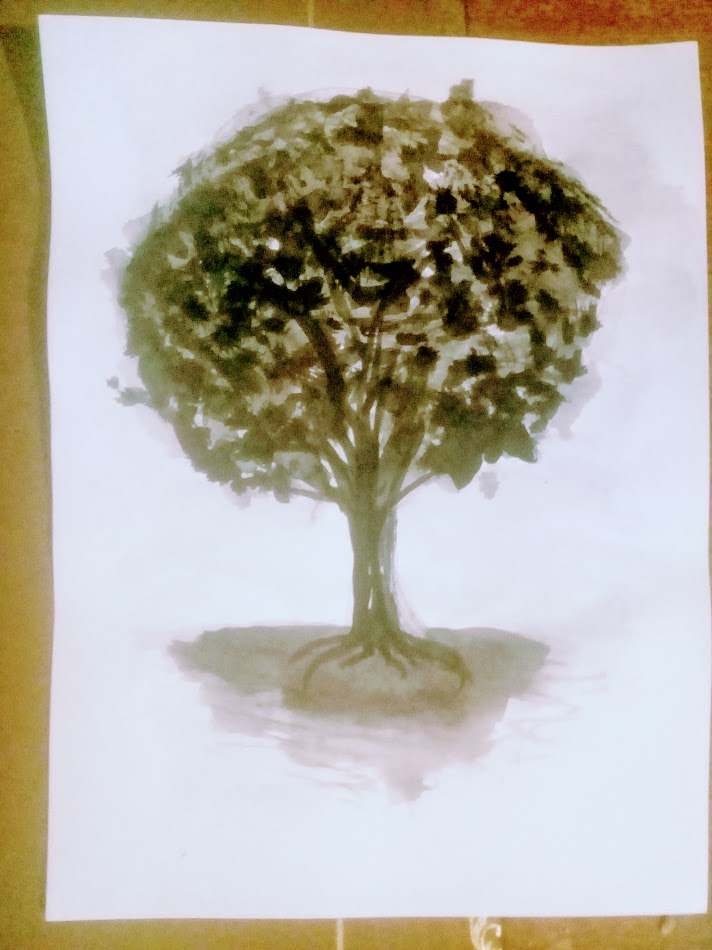
\includegraphics[width=.5\textwidth,trim=1.9cm 2cm 1.5cm 1.6cm,clip]{arbol_tilo}
\end{wrapfigure}

\begin{flushleft}
	ESPERÉ UN RATO, NO PODRÍA BAJAR CON ESAS DOS
	
	 PERRITAS 	SUELTAS. Y PARA PODER DESCENDER, 
	 
	 NECESITABA ALGO ENTRE EL ALTO MURO Y EL PISO. 
	
	PENSÉ EN LOS ÁRBOLES DE TILO QUE ESTÁN 
	
	JUNTO A LA CASA. SON MUY LINDOS, DE COPAS CON MUCHAS HOJAS EN PRIMAVERA, Y HOJAS QUE CAEN, JUNTO A SEMILLAS DURANTE EL OTOÑO. MUCHAS DE ELLAS CAEN EN NUESTRO PATIO Y JUEGO UN POCO CON LAS SEMILLAS.
	
	SIEMPRE ME DICEN QUE PAREZCO UNA PEQUEÑA PANTERA 
	
	NEGRA$\ldots$ ERA HORA DE DEMOSTRARLO.
	
\end{flushleft}
\newpage
 
\tikz[remember picture,overlay] \node[opacity=0.8,inner sep=0pt] at (current page.center){
\includegraphics[width=\paperwidth,height=\paperheight,angle=180]{paper3}};
\begin{minipage}{.9\textwidth}
	DURANTE MI SIESTA YA HABÍA PENSADO EN EL SALTO. A MENUDO PIENSO EN MIS PROEZAS FELINAS A LA HORA DE DORMIR, ASÍ ME DUERMO CON UNA SONRISA.
\end{minipage}
\begin{figure}[h]
\centering
	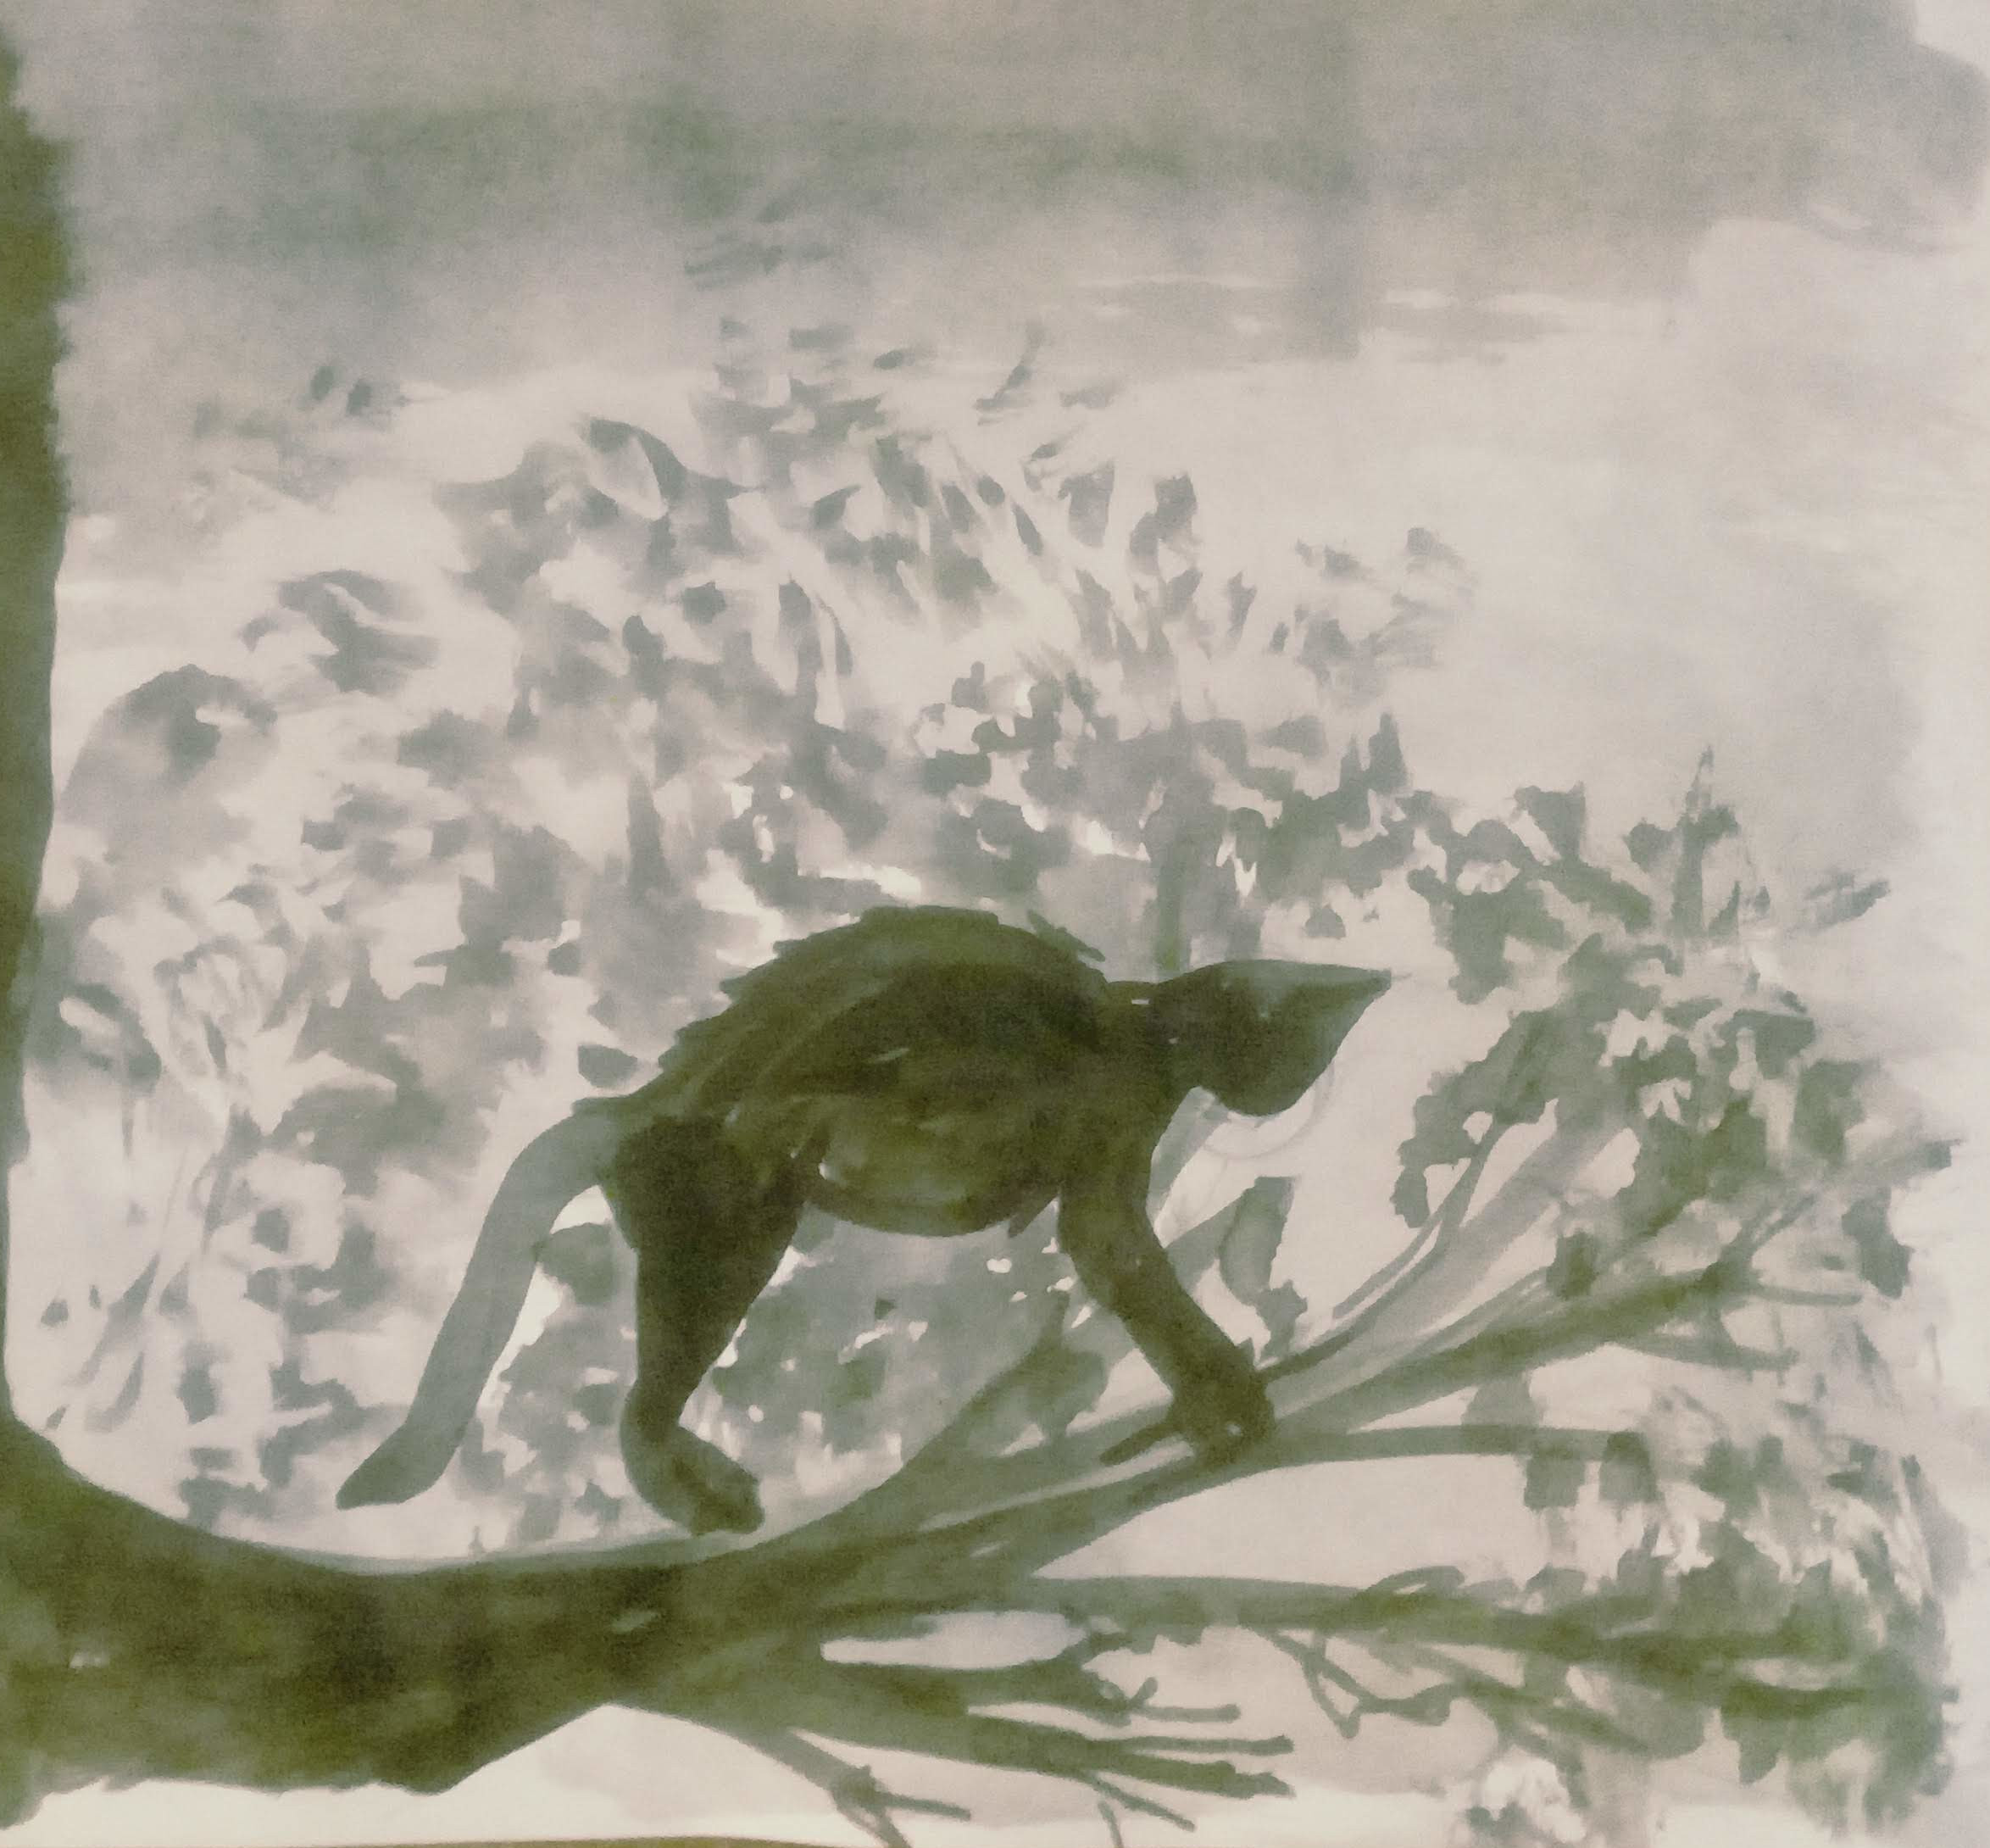
\includegraphics[width=.5\textwidth,trim=0cm 0cm 0cm 5cm,clip]{arriba_arbol}
\end{figure}	

\begin{minipage}{.9\textwidth}	
	PERO AHORA, BIEN DESPIERTO, NO IBA A FALLAR NINGÚN CÁLCULO. TODO MI ENTRENAMIENTO EN EL PATIO, TREPANDO EN LA BIBLIOTECA, SOBRE EL PIANO, SOBRE LA SILLA ALTA$\ldots$ TODO IBA A SERVIRME EN MI CAIDA CON ESTILO SOBRE LA RAMA. Y ASÍ FUE, UNA MANIOBRA LIMPIA Y DISTINGUIDA, SÉ QUIENES ESTARÍAN ORGULLOSOS DE MÍ. 
\end{minipage}
\newpage

\tikz[remember picture,overlay] \node[opacity=0.8,inner sep=0pt] at (current page.center){
\includegraphics[width=\paperwidth,height=\paperheight,angle=180]{paper3}};
\begin{minipage}{.49\textwidth}
	YA CAMINANDO POR LA VEREDA, DESDE AFUERA, LA CASA SE VEÍA MÁS GRANDE. VI ACERCARSE UN PERRO Y VOLVÍ A TREPARME AL ÁRBOL SIN PROBLEMAS
	
	AHORA QUE ME HABÍA OLVIDADO DE LAS PALOMAS, DI UNA VUELTA A LA PEQUEÑA MANZANA QUE CONTIENE A MI CASA. YA HABÍA VISTO UN POCO LA CALLE CUANDO ME HABÍAN LLEVADO A VACUNAR. PERO, ¿QUÉ DIRECCIÓN TOMAR? DECIDÍ IR HACIA DONDE VIERA PERSONAS, PUES PODÍA SER INTERESANTE APRENDER ALGO NUEVO. FUI AVANZANDO DE POCO ESCONDIÉNDOME PRIMERO EN UN CANTERO, LUEGO DETRÁS DE UNAS PALMERAS.
\end{minipage}\hfill
 \begin{minipage}{.43\textwidth}
	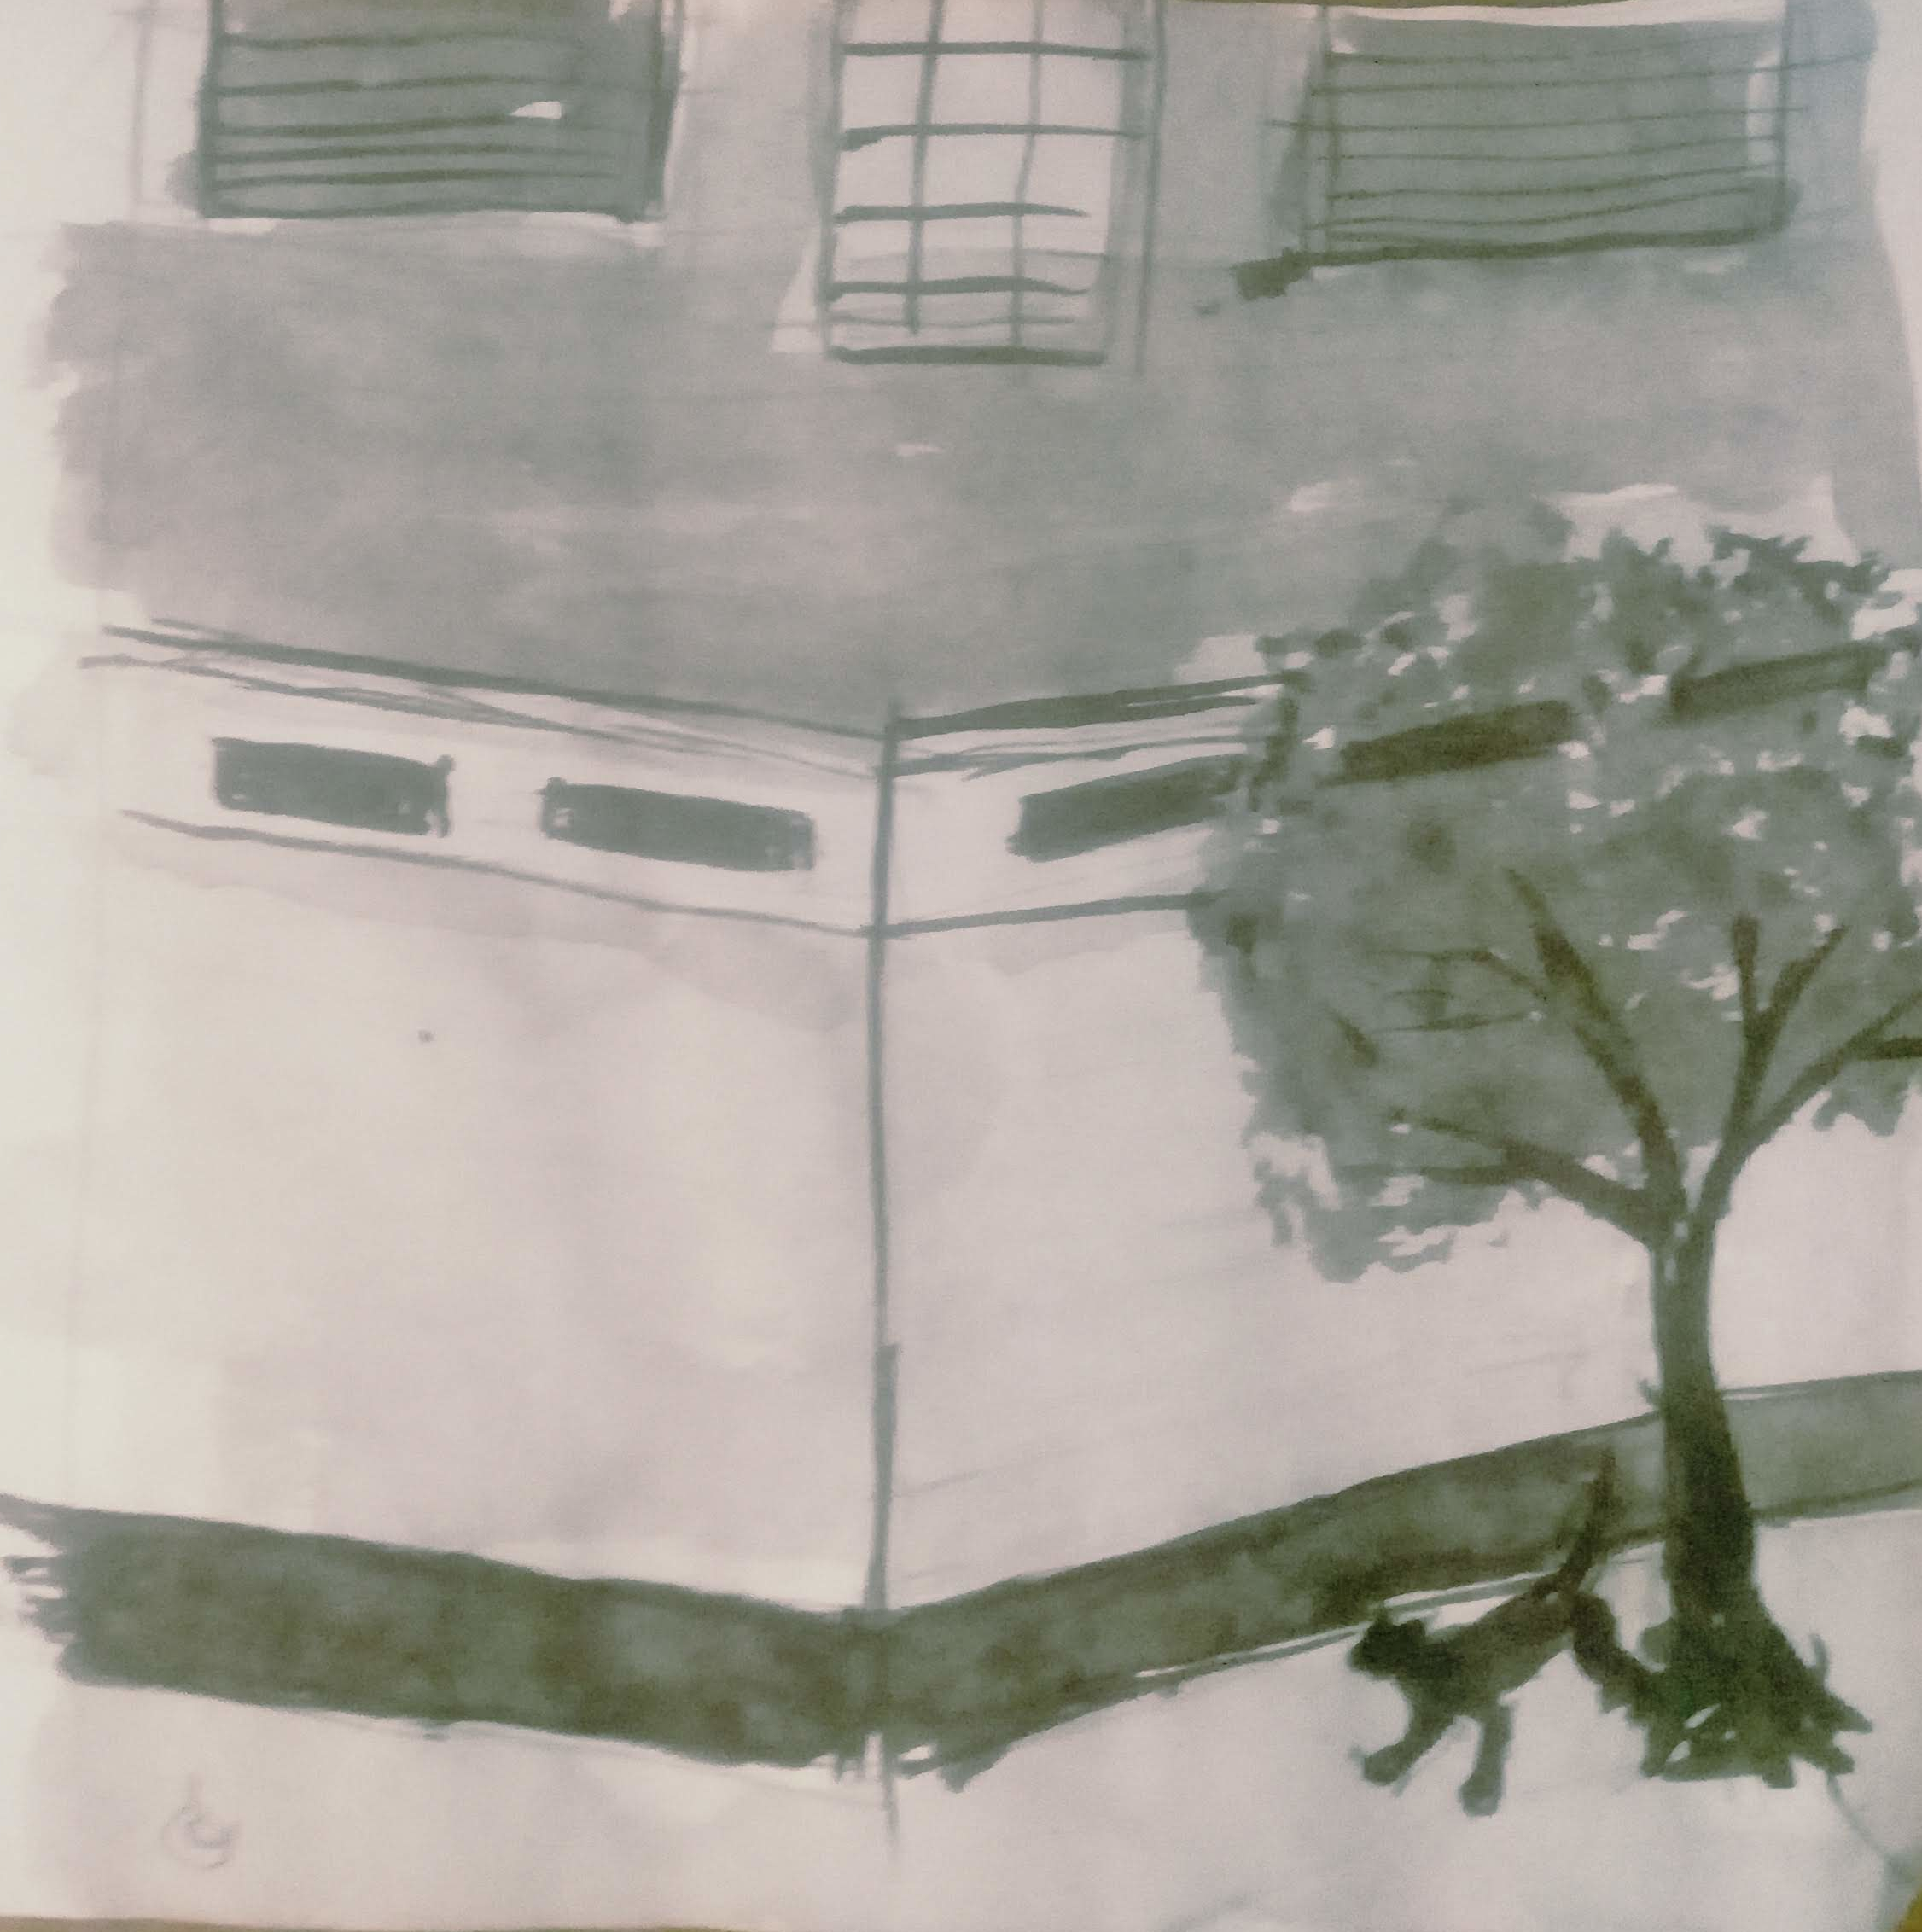
\includegraphics[width=\textwidth,trim=1cm 0cm 0cm 0cm,clip]{vereda1}
\end{minipage}

\newpage

\tikz[remember picture,overlay] \node[opacity=0.8,inner sep=0pt] at (current page.center){
\includegraphics[width=\paperwidth,height=\paperheight,angle=180]{paper4}};
\begin{minipage}{.49\textwidth}
	IBA A TENER QUE CRUZAR LA CALLE. ES UNA SENSACIÓN DISTINTA, PUES YA LA SUPERFICIE NO ES LA MISMA QUE LA VEREDA Y HAY UNA BAJADITA, QUE LLAMAN ``CORDÓN''. EN GENERAL HAY ASFALTO, QUE ES UNA SUPERFICIE LISA Y UN PUCO RUGOSA A LA VEZ. EN OCASIONES, SE CONSERVAN DESDE LA ÉPOCA DE CUANDO MI PAPÁ ERA CHIQUITO, LOS ADOQUINES. SON COMO PIEDRAS TODAS DEL MISMO TAMAÑO, ORDENADAS REGULARMENTE. SON MUY DUROS Y LISOS, AUNQUE LOS AUTOS CUANDO PASAN HACEN MUCHO RUIDO PORQUE LES DAN COMO GOLPECITOS. 
	
	

\end{minipage}\hfill
\begin{minipage}{.43\textwidth}
	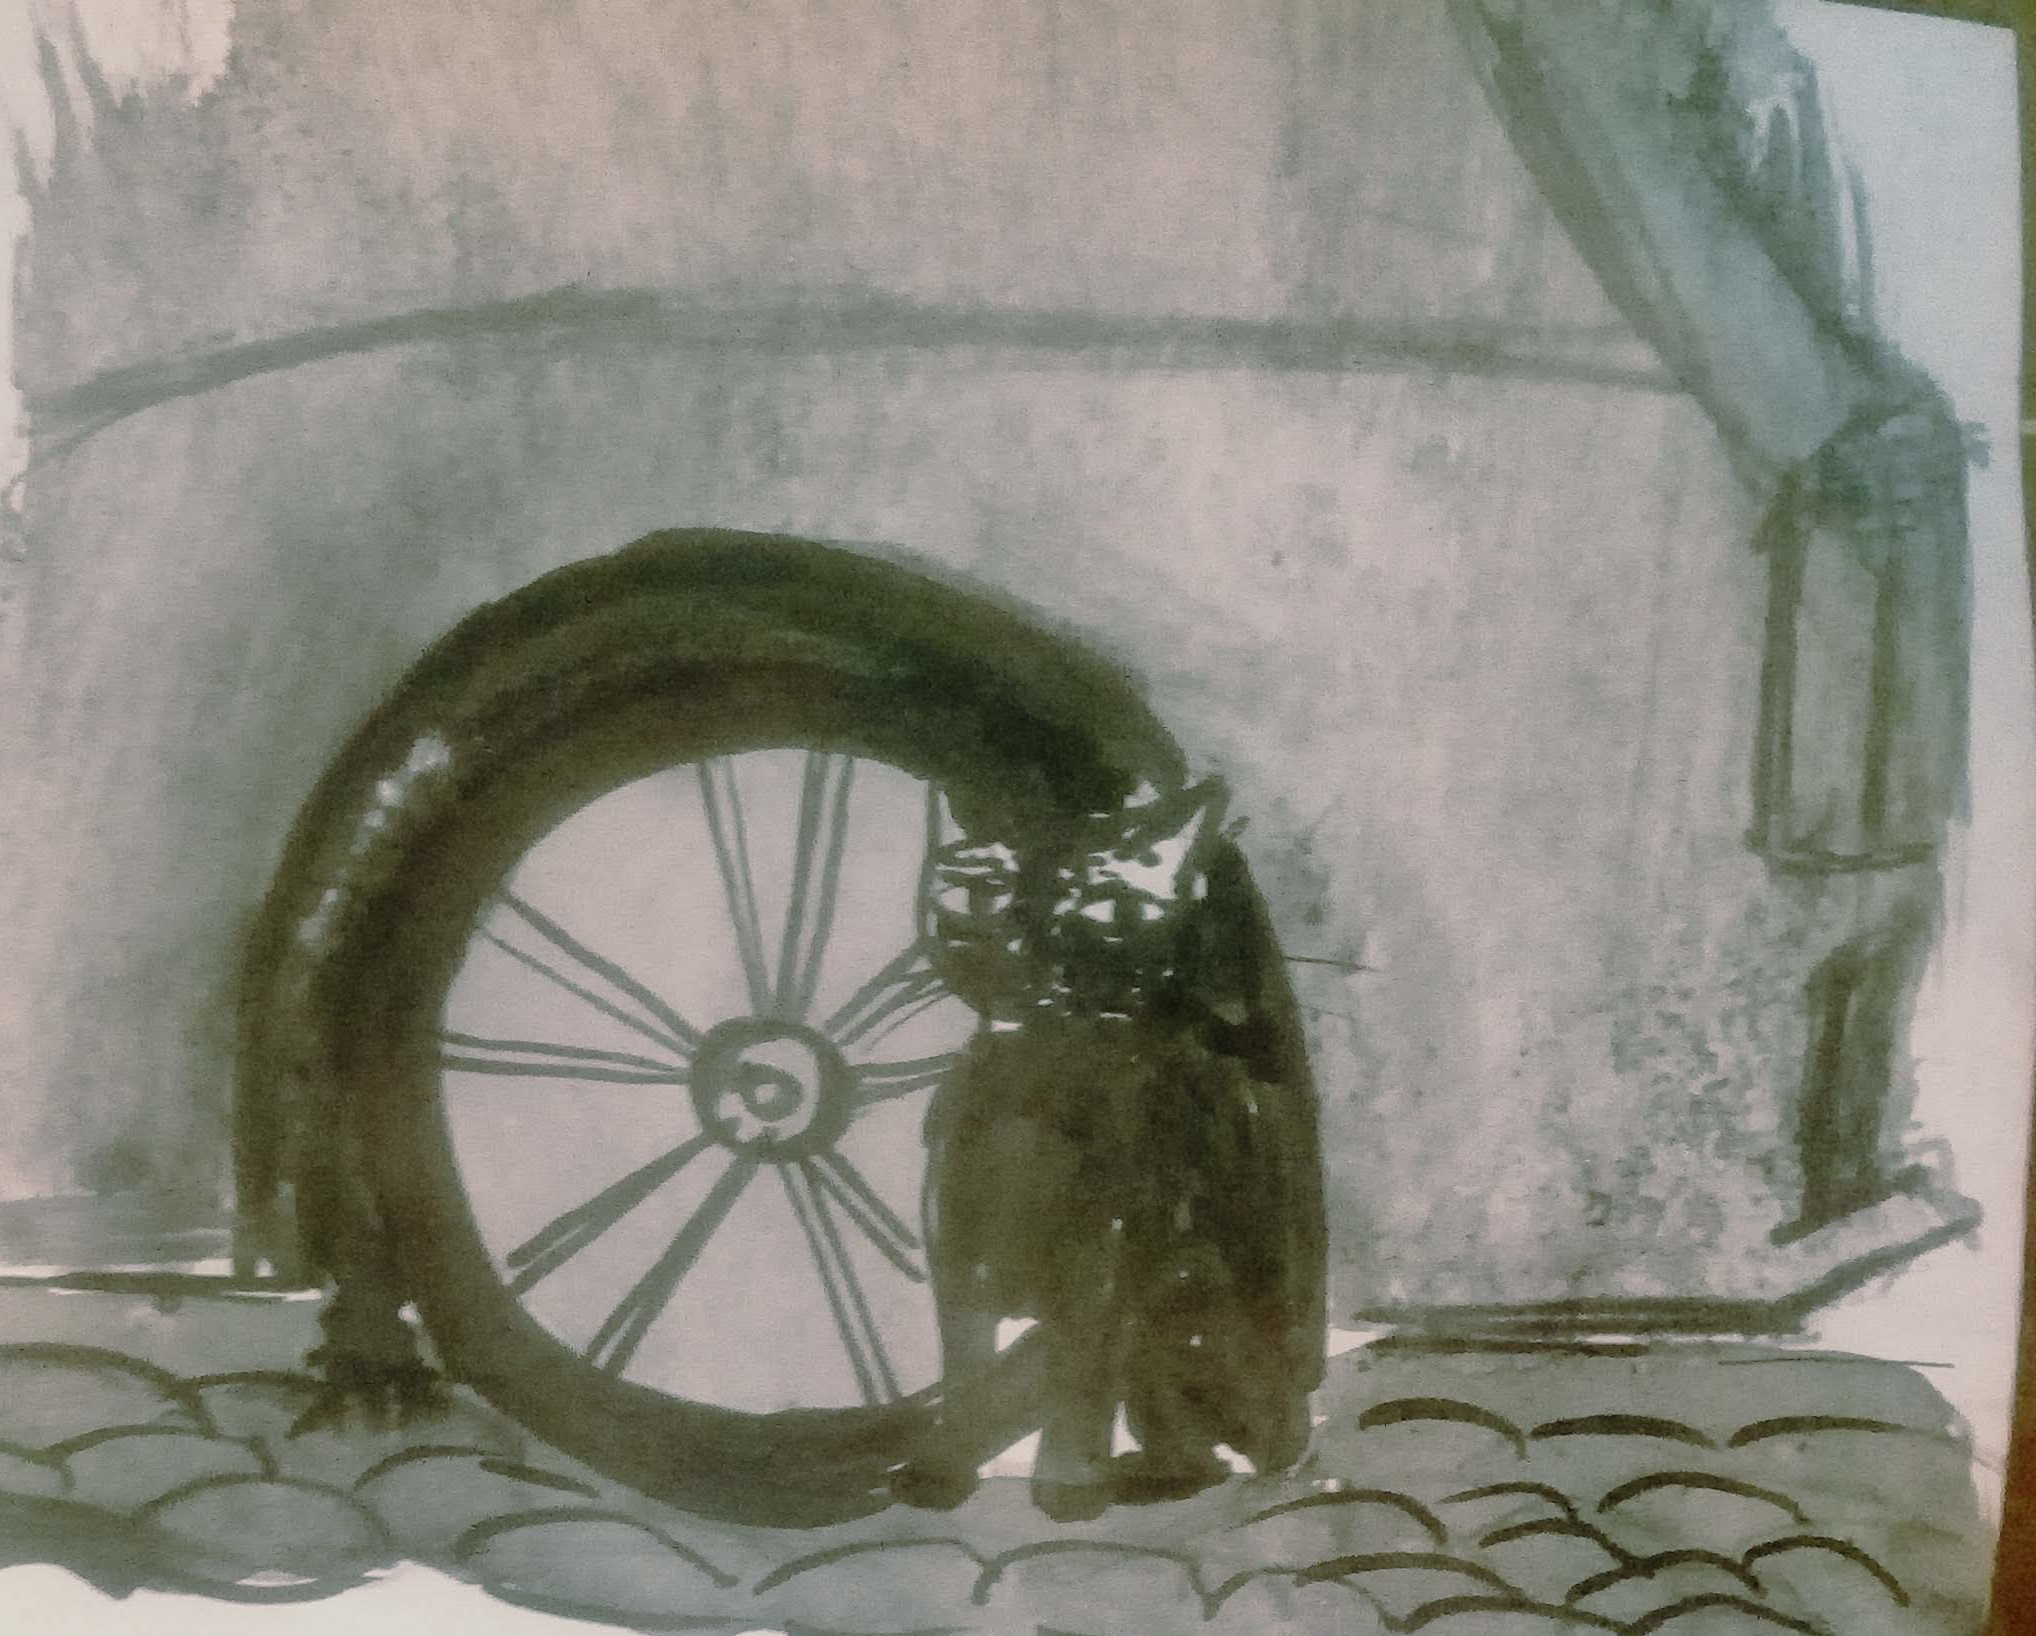
\includegraphics[width=\textwidth,trim=1cm 0cm 0cm 0cm,clip]{rueda_auto}
	
	ANTES DE IR SOBRE LA CALLE, ME DETUVE UNOS INSTANTES AL COSTADO DE UNA RUEDA DE AUTO.
\end{minipage}

\newpage
		\xsavebox{PageBGPicture}{%
	\begin{tikzpicture}
	\node [ minimum width=.\paperwidth, minimum height=\paperheight] () {
\includegraphics[width=\paperwidth,height=\paperheight,angle=180]{paper5}};
	\end{tikzpicture}
}
\pagenumbering{gobble}
\tikz[remember picture,overlay] \node[opacity=1,inner sep=0pt] at (current page.center){
\includegraphics[width=\paperwidth,height=\paperheight,angle=180]{paper5}};
\begin{minipage}{\textwidth}
	ATRAVASÉ LA CALLE DE ADOQUINES MIRANDO BIEN QUE NO HUBIERA NINGÚN AUTO EN MOVIMIENTO.  NI BIEN LLEGUÉ A LA OTRA VEREDA, PERCIBÍ UN AROMA DELICIOSO. YA LO HABÍA SENTIDO ANTES, HACE UNOS MESES, CREO QUE SE TRATABA DE COMIDA CHINA: CHAW FAN Y BUÑUELOS DE POLLO!
 \begin{wrapfigure}{r}{.6\textwidth}
	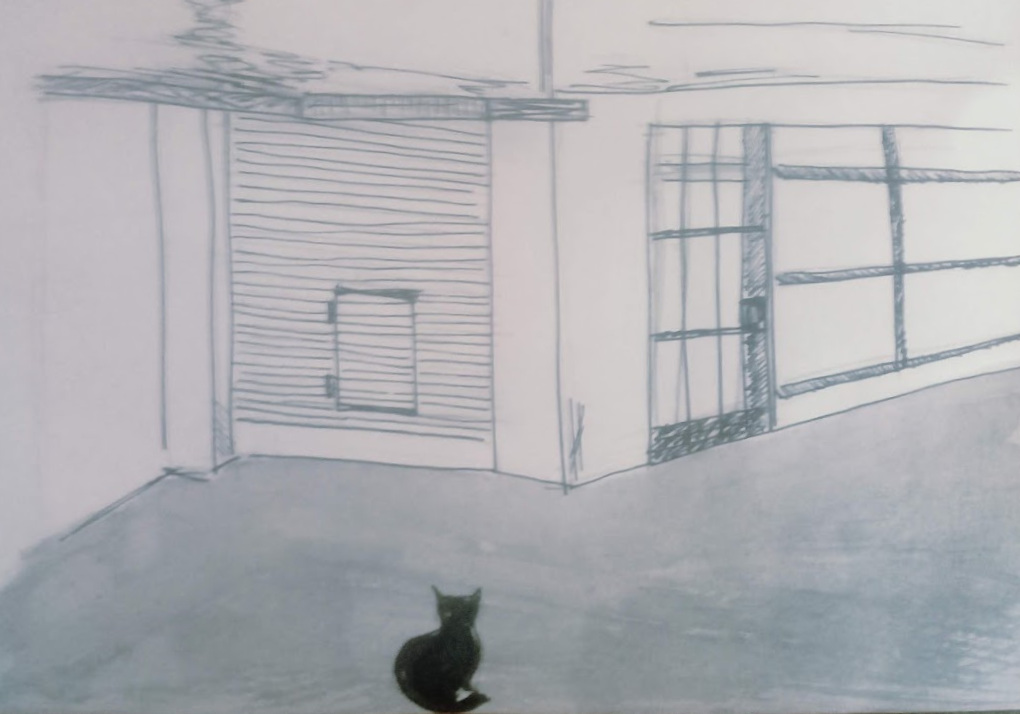
\includegraphics[width=.6\textwidth,trim=0cm 0cm 0cm 0cm,clip]{comida_china}
\end{wrapfigure}
	PERO NO VEÍA NADA MÁS QUE UNA PERSIANA DE METAL BAJA Y AL LADO UNA PUERTA CERRADA. AGUCÉ MI OÍDO FELINO Y ESCUCHÉ MOVIMIENTO DE PERSONAS AL INTERIOR. ESCUCHÉ UN AUTO ACERCARSE Y ME DÍ VUELTA. SE TRATABA DE UN AUTO CON LUCES PARPADEANTES AZULES Y SE DETUVO JUSTO A METROS DE DONDE YO ESTABA. DE UN SALTO ME PUSE A UNA BUENA DISTANCIA A OBSERVAR. 
	BAJÓ UN SEÑOR QUE VESTÍA UN UNIFORME AZUL OSCURO, Y RÁPIDAMENTE SE ACERCÓ A LA PERSIANA BAJA. 

	
\end{minipage}

\newpage
\xsavebox{PageBGPicture}{%
	\begin{tikzpicture}
		\node [ minimum width=.\paperwidth, minimum height=\paperheight] () {
\includegraphics[width=\paperwidth,height=\paperheight,angle=180]{paper6}};
	\end{tikzpicture}
}
\pagenumbering{gobble}
\tikz[remember picture,overlay] \node[opacity=1,inner sep=0pt] at (current page.center){
\includegraphics[width=\paperwidth,height=\paperheight,angle=180]{paper6}};
\begin{minipage}{\textwidth}
	EL UNIFORMADO GOLPEO ŔAPIDO TRES VECES CON LA MITAD DE SU DEDO ÍNDICE EN LA PERSIANA. 
	\begin{wrapfigure}{r}{.57\textwidth}
		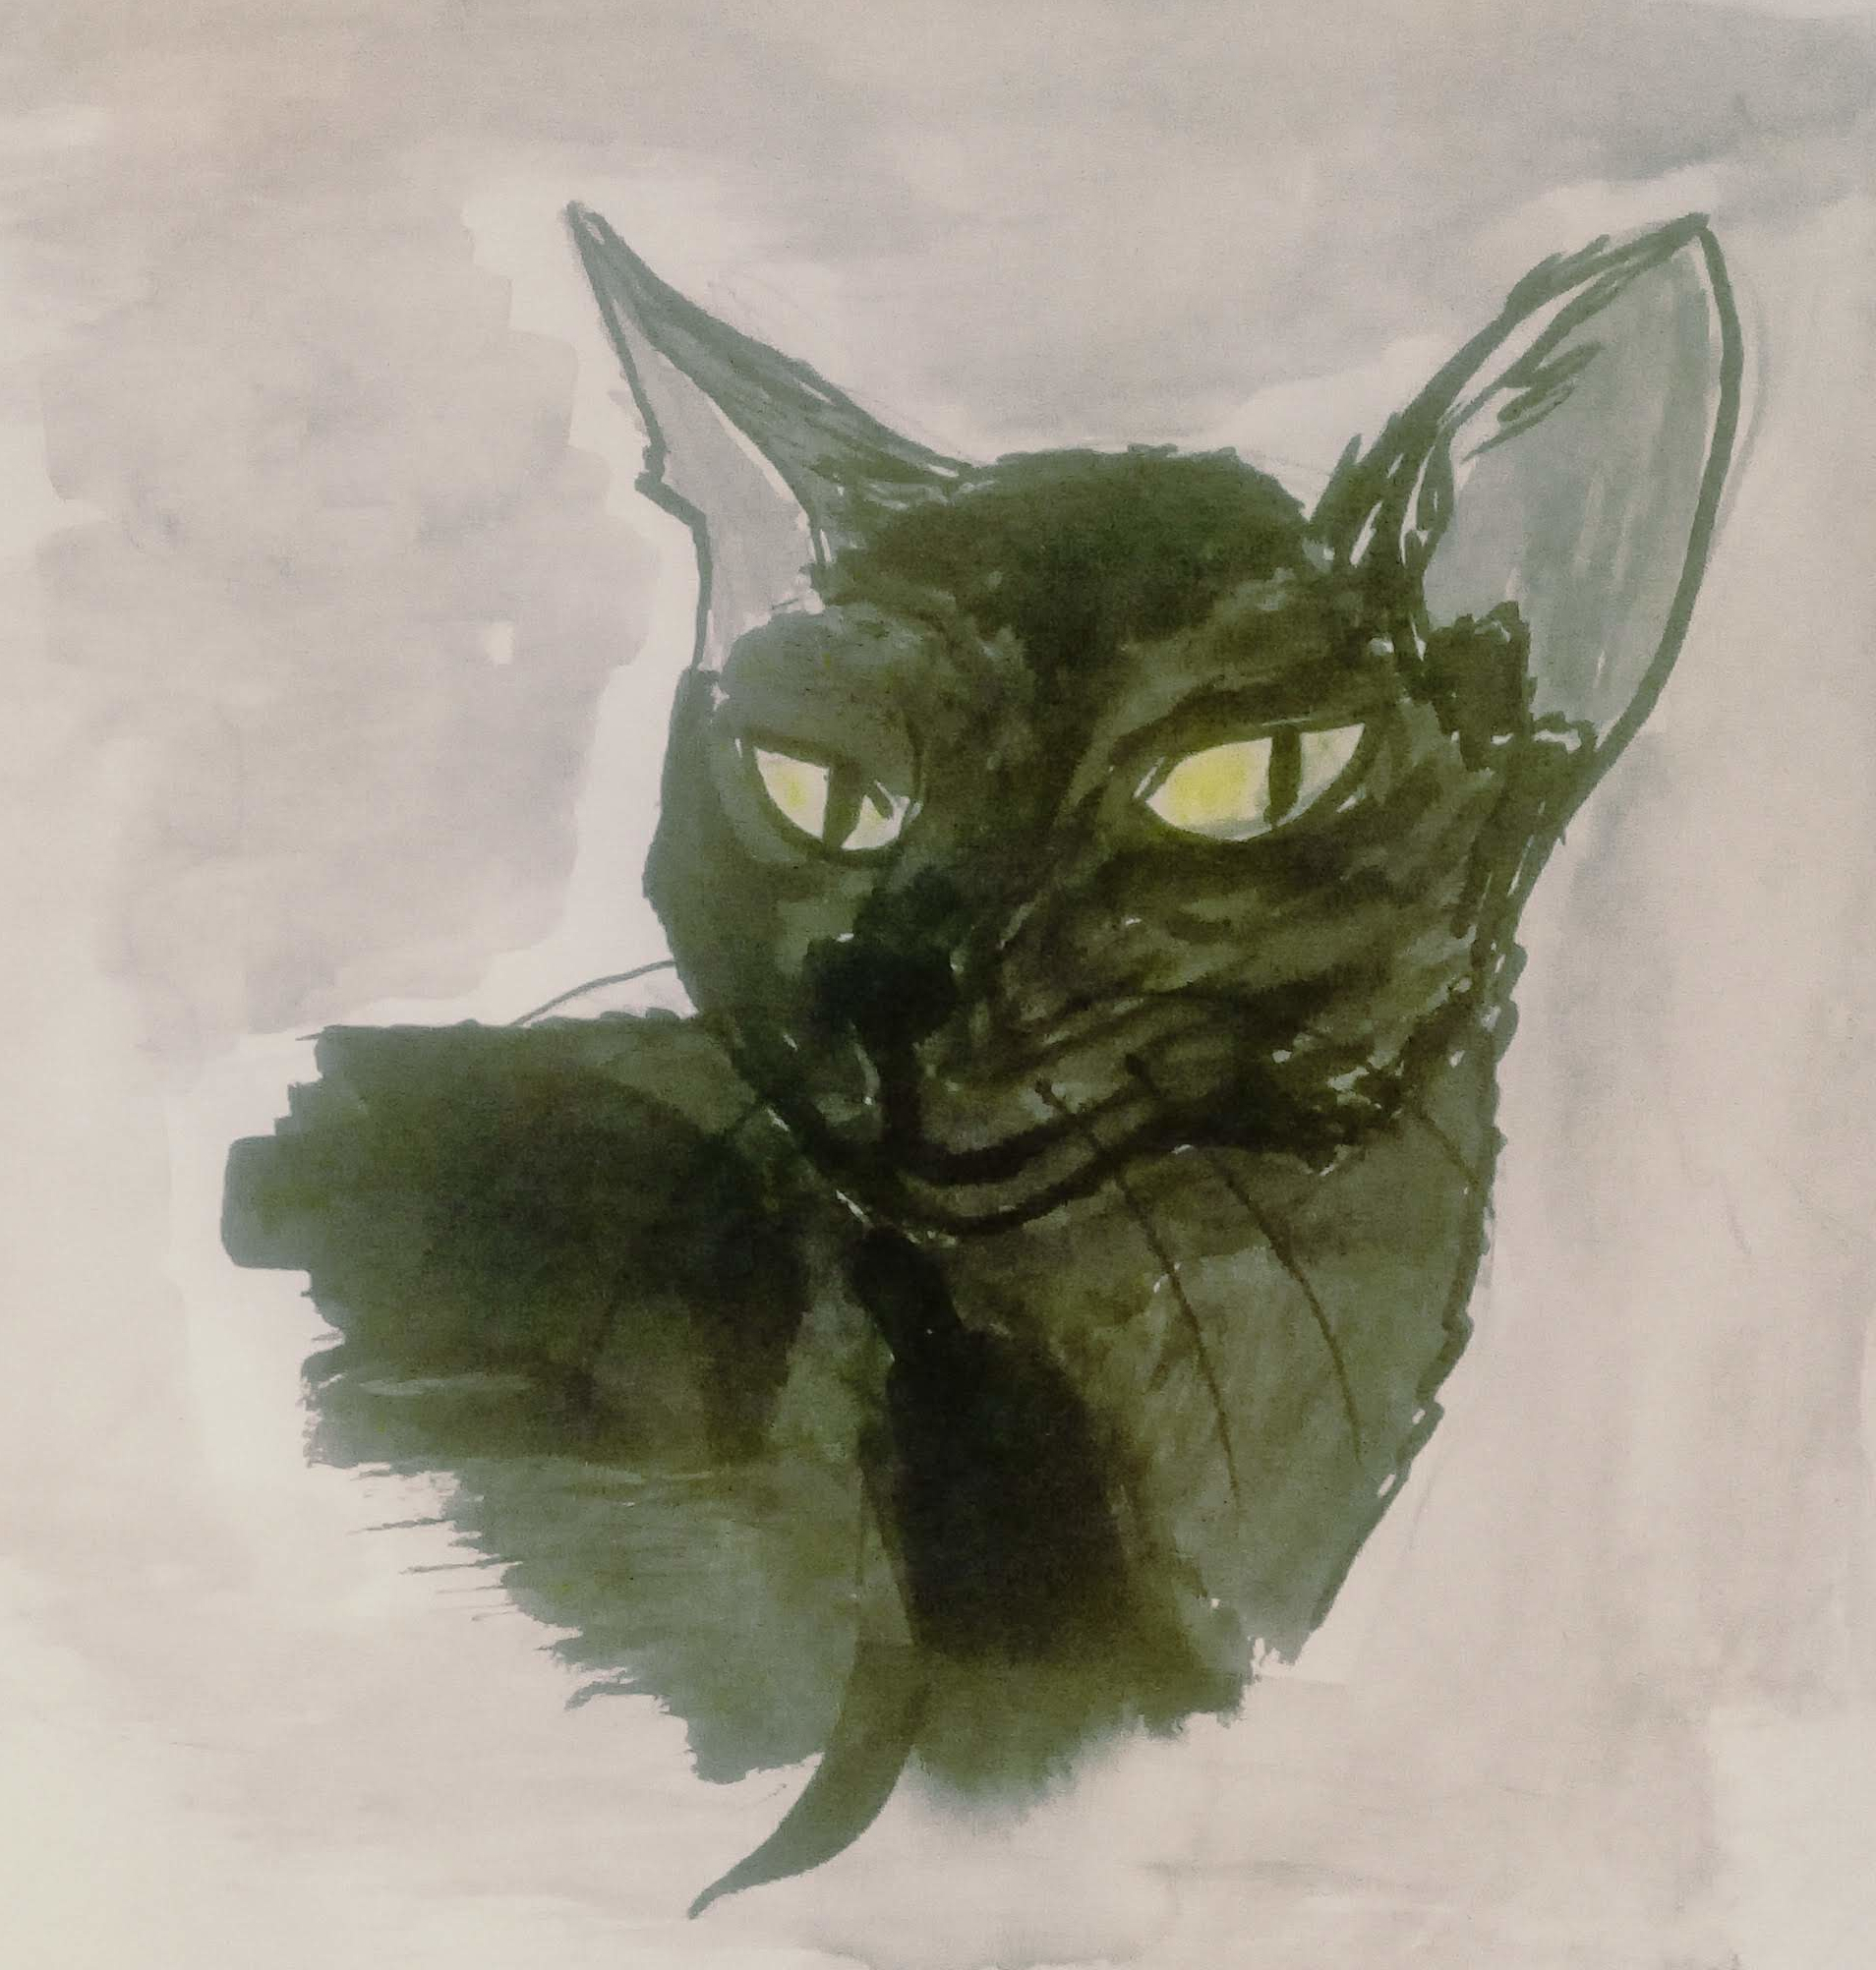
\includegraphics[width=.57\textwidth,trim=0cm 0cm 0cm 0cm,clip]{frente_al_chino}
	\end{wrapfigure}
DE PRONTO, UNA PEQUEÑA PUERTA SE ABRIÓ Y UN BRAZO ASOMÓ CON LO QUE IMAGINO ERA UN BANQUETE FENOMENAL DE COMIDA CHINA. POR UN INSTANTE MEDÍ LAS POSIBILIDADES DE ROBAR GRACIAS A MIS PODEROSOS RECURSOS FELINOS. MÁS DE UNA VEZ HABÍA CONSEGUIDO EN CASA PEDACITOS DE JAMÓN, DE QUESO, DE PIZZA, DE POLLO, BUENO, ¡Y ALGUNA COSA MÁS DE LA QUE AÚN NO SE DIERON CUENTA!

SEGUÍA LOS MOVIMIENTOS EN TORNO A LA COMIDA CUANDO MIS SENTIDOS GATUNOS ME INDICARON QUE OTRO HUMANO SE ACERCABA. MIRÉ CON EL COSTADO DE MIS OJOS Y ALCANCÉ A DETECTAR UNA SEÑORA DE VOZ ALGO ESTRIDENTE ¡QUE PARECÍA QUE ME HABLABA A MÍ!
	
	
\end{minipage}
\end{document}
